\section{Fonctions et modules}

	\subsection{Théorème de Pythagore} \label{corr:pythagore} (Énoncé~: \ref{appl:pythagore})
	
		On a le programme suivant~:
		\begin{pythoncode}
				# On créé une fonction qui prend trois arguments
				def pythagore(a, b, c):
					# Si la somme des carrés des deux côtés est égale au carré du troisième
					if (a ** 2) + (b ** 2) == (c ** 2):
						return True
					# Sinon
					else:
						return False
			\end{pythoncode}
	
	\subsection{Implémentation de la fonction factorielle} \label{corr:factorielle} (Énoncé~: \ref{appl:factorielle})
		
		Il y a $n$ tour de boucle à faire, l'utilisation d'une boucle itérative s'impose~:
		\begin{pythoncode}
			def factorielle(n):
				resultat = 1
				for i in range(1, n + 1):
					resultat = resultat * i
				return resultat
		\end{pythoncode}

	\subsection{Test de la primalité d'un nombre} \label{corr:premier} (Énoncé~: \ref{appl:premier})
	
		En reprenant les étapes données, on obtient~:
		\begin{pythoncode}
			from math import sqrt
	
			def premier(p):
				for n in range(2, int(sqrt(p)) + 1):
					if p % n == 0:
						return False
				return True
		\end{pythoncode}
	
	\subsection{Version récursive de l'algorithme d'Euclide} \label{corr:euclide_rec} (Énoncé~: \ref{appl:euclide_rec})
		
		Le programme récursif va s'axer autour de la condition $b = 0$. En effet si $b$ est nul, le PGCD de $a$ et $b$ est $a$, sinon $PGCD(a~;\ b) = PGCD(b~;\ a \ MOD\ b)$. Ainsi~:
		\begin{pythoncode}
			def pgcd(a, b):
				if b == 0:
					return a
				else:
					return pgcd(a, a % b)
		\end{pythoncode}

\section{Outils pour l'ingénierie numérique}
	
	\subsection{Calcul des points d'une fonction et affichage} \label{corr:pts_fonction} (Énoncé~: \ref{appl:pts_fonction})
	
		En choisissant de représenter $f~:\ x \mapsto \frac{\sin(x)}{x}$ sur l'intervalle $[0.5~;\ 5]$ avec 1000 points~:
		\begin{pythoncode}
			from math import sin
			import matplotlib.pyplot as plt
			import numpy as np
			
			# Définition de la fonction f
			def f(x):
				return sin(x) / x
			
			# Calcul automatique des abcisses
			X = np.linspace(0.5, 5, 1000)
			
			# Construction des ordonnées
			Y = np.vectorize(f)(X)
			
			# Affichage du résultat
			plt.plot(X, Y)
			plt.show()
		\end{pythoncode}
		\begin{figure}[h]
			\centering
			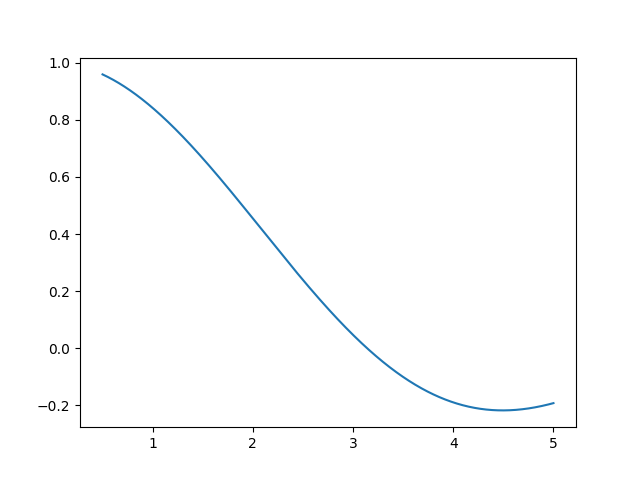
\includegraphics[scale=0.60]{images/Figure_2.png}
			\caption{$f(x)$ sur $[0.5~;\ 5]$}
		\end{figure}

\section{Algorithmes usuels}
	
	\subsection{Courbe d'une solution d'une équation différentielle} \label{corr:equa_diff} (Énoncé~: \ref{appl:equa_diff})
		
		On veut tracer une solution de cette équation différentielle~:
		\[
			\forall t \in [-1~;\ 10],\ (t^2 + 1)y' + (t - 1)^2y = t^3 - t^2 + t + 1
		\]
		Avec la condition initiale~: $y(-1) = 8$.
		
		En reprenant point par point~:
		\begin{enumerate}
			\item Assez simplement, on isole $y'$~:
			\[ \begin{array}{rll}
				(t^2 + 1)y' + (t - 1)^2y & = & t^3 - t^2 + t + 1 \\
				(t^2 + 1)y' & = & t^3 - t^2 + t + 1 - (t - 1)^2y \\
				y' & = & \frac{1}{(t^2 + 1)} \cdot (t^3 - t^2 + t + 1 - (t - 1)^2y)
			\end{array} \]
			Ainsi, on pose $\forall t \in [-1~;\ 10],\ y' = f(t, y) = \frac{1}{(t^2 + 1)} \cdot (t^3 - t^2 + t + 1 - (t - 1)^2y)$
			\begin{pythoncode}
				def f(t, y):
					return (1 / (t**2 + 1)) * (t**3 - t**2 + t + 1 - (t - 1)**2 * y)
			\end{pythoncode}
			
			\item On se place sur l'intervalle $[-1~;\ 10]$ avec un nombre arbitraire de points, on peut prendre $N = 1000$. Ainsi,
			\begin{pythoncode}
				h = (10 + 1) / 1000
				X = [-1 + n * h for n in range(1000)]
			\end{pythoncode}
			
			\item On initialise les ordonnées avec la condition initiale et on complète la liste~:
			\begin{pythoncode}
				Y = [8]
				for i in range(1000 - 1):
					Y.append(Y[i] + h * f(X[i], Y[i]))
			\end{pythoncode}
			
			\item Il ne reste plus qu'à tracer et à afficher~:
			\begin{pythoncode}
				plt.plot(X, Y)
				plt.show()
			\end{pythoncode}
		\end{enumerate}
	
	En résumé, le code complet~:
	\begin{pythoncode}
		import matplotlib.pyplot as plt
		
		def f(t, y):
			return (1 / (t**2 + 1)) * (t**3 - t**2 + t + 1 - (t - 1)**2 * y)
		
		h = (10 + 1) / 1000
		X = [-1 + n * h for n in range(1000)]
		
		Y = [8]
		for i in range(1000 - 1):
			Y.append(Y[i] + h * f(X[i], Y[i]))
		
		plt.plot(X, Y)
		plt.show()
	\end{pythoncode}
	
	La figure de gauche représente la solution de condition initiale $y(-1) = 8$ sur l'intervalle $[-1~;\ 10]$ et la figure de droite représente les solutions approchées pour des valeurs initiales entre $0$ et $8$ et $t$ entre $-1$ et $3$.
	
	\begin{tabular}{cc}
		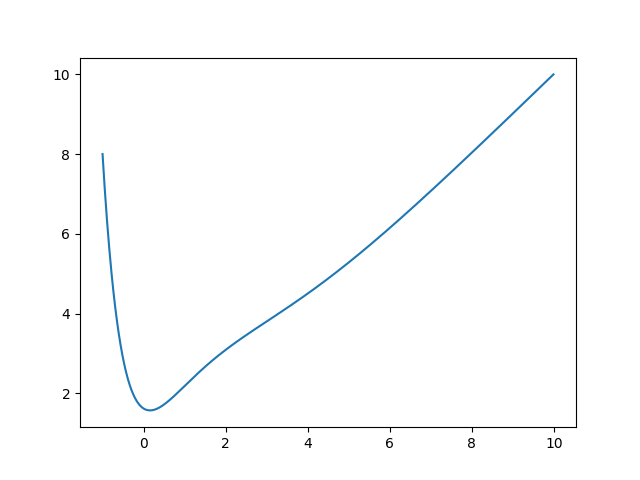
\includegraphics[scale=0.50]{images/Figure_5.png} &
		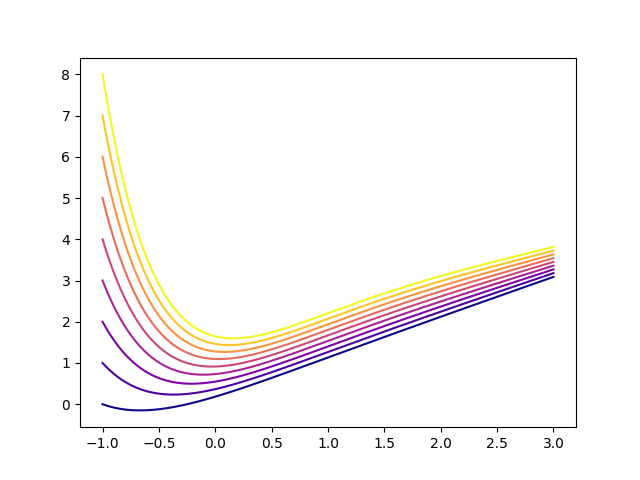
\includegraphics[scale=0.50]{images/Figure_6.png} \\
	\end{tabular}

\section{Programmation orientée objet}

	\subsection{Vecteurs} \label{corr:vecteurs} (Énoncé~: \ref{appl:vecteurs})
		
		\subsubsection{Initialisze l'objet}
		Le plus simple pour représenter un vecteur est d'utiliser une liste Python contenant les composantes du vecteurs selon les différentes coordonnées. Ainsi l'initialisation du vecteur va ressembler à~:
		\begin{pythoncode}
			class Vecteur:
				def __init__(self, composantes):
					self.composantes = composantes
					self.taille = len(composantes) # on stocke aussi la dimension du vecteur
		\end{pythoncode}
		
		\subsubsection{Afficher l'objet}
		Commencer par programmer l'affichage du nouvel objet permet de faire des tests assez rapidement ce qui est agréable. Ici rien de très compliqué.
		
		On pourrait transtyper deux fois notre liste de coordonnées~: une première fois pour avoir un tuple et une seconde fois pour avoir une chaîne de caractères. Cette solution fonctionne, mais n'est pas très élégante. Il est préférable de construire directement la représentation de l'objet~:
		\begin{pythoncode}
			def __repr__(self):
				composantes_str = [str(i) for i in self.composantes] # on construit la liste des composantes sous forme de chaînes de caractères
				return "(" + ", ".join(composantes_str) + ")"
		\end{pythoncode}
		
		\subsubsection{Addition de deux vecteurs}
		L'addition sur les vecteurs est une addition terme à terme, donc rien de très compliqué~:
		\begin{pythoncode}
			def __add__(self, vecteur):
				if self.taille != vecteur.taille:
					raise ValueError("on ne peut pas sommer deux vecteurs de tailles différentes") # On arrête l'exécution du programme et on renvoie une erreur de valeur
				
				resultat = [] # les composantes du nouveau vecteur
				for i in range(self.taille):
					resultat.append(self.composantes[i] + vecteur.composantes[i])
				
				return Vecteur(resultat) # on renvoie une instance de la classe Vecteur
		\end{pythoncode}
		
		\subsubsection{Multiplication par un scalaire}
		La multiplication entre un vecteur et un scalaire est simple~: chaque composante du vecteur est multipliée par le scalaire.
		\begin{pythoncode}
			def __mul__(self, scalaire):
				if not isinstance(scalaire, (int, float)):
					raise TypeError("ce n'est pas un scalaire") # si 'sclaire' n'est ni un int, ni un float, on arrête l'exécution du programme et on renvoie une erreur de type
				
				resultat = []
				for i in range(self.taille):
					resultat.append(scalaire * self.composantes[i])
				
				return Vecteur(resultat)
		\end{pythoncode}
		
		\subsubsection{Résumé et idées pour aller plus loin}
		Le code complet du vecteur est donc~:
		\begin{pythoncode}
			class Vecteur:
				def __init__(self, composantes):
					self.composantes = composantes
					self.taille = len(composantes)
					
				def __repr__(self):
					composantes_str = [str(i) for i in self.composantes]
					return "(" + ", ".join(composantes_str) + ")"
								
				__str__ = __repr__
				
				def __add__(self, vecteur):
					if self.taille != vecteur.taille:
						raise ValueError("on ne peut pas sommer deux vecteurs de tailles différentes")
					
					resultat = []
					for i in range(self.taille):
						resultat.append(self.composantes[i] + vecteur.composantes[i])
					
					return Vecteur(resultat)
				
				__radd__ = __add__
					
				def __mul__(self, scalaire):
					if not isinstance(scalaire, (int, float)):
						raise TypeError("ce n'est pas un scalaire")
					
					resultat = []
					for i in range(self.taille):
						resultat.append(scalaire * self.composantes[i])
					
					return Vecteur(resultat)
				
				__rmul__ = __mul__
		\end{pythoncode}
		
		Bien sûr il existe d'autres manipulations sur les vecteurs~: produit scalaire, norme, produit vectoriel etc. Ces fonctions ne sont pas expliquées ici, mais sont tout à fait faisables.
	
	\subsection{Polynômes} \label{corr:polynomes} (Énoncé~: \ref{appl:polynomes})
		
		\subsubsection{Initialiser l'objet}
		Avant d'écrire les méthodes, il faut penser à la manière dont l'objet va être représenté dans la classe. Ici, un polynôme est entièrement caractérisé par la donnée de ses coefficients, ainsi le polynôme va devoir avoir un attribut \python|coefficients| qui sera une liste. Le premier élément de la liste correspondra au coefficient de puissance nulle (indice 0 dans la liste), le second élément (indice 1) sera le coefficient de degré 1 etc.
		
		On impose par ailleurs un attribut \python|deg| qui correspond au degré du polynôme. Le degré correspond à la puissance maximale, de coefficient non nul. En supposant que la liste ne finit pas par un $0$, il s'agit de la longueur de la liste moins un.
		
		Avec les deux derniers paragraphes, on peut déjà rédiger la méthode \python|__init__|~:
		\begin{pythoncode}
			class Polynome:
				def __init__(self, coefficients):
					self.coefficients = coefficients
					self.deg = len(coefficients) - 1
		\end{pythoncode}
		
		\subsubsection{Afficher un polynôme}
		L'affichage maintenant. La liste des coefficients est triée par ordre croissant de puissance, donc le polynôme va être affiché dans cet ordre (on aurait pu l'afficher dans l'autre sens, mais cela ne présente pas beaucoup d'intérêt ici). L'idée va être de décomposer le polynôme en une liste de chaîne de caractères où chaque élément est un monôme qui compose le polynôme.
		
		Nous allons donc reccourir à une liste \python|monomes|. Ensuite, il va falloir faire une boucle \python|for| qui balaye les coeffiicents du polynôme à afficher en distinguant les cas~:
		\begin{itemize}
			\item si le coefficient vaut $0$, il n'y a rien à afficher
			\item si la puissance vaut $0$, $X^0 = 1$
			\item si la puissance vaut $1$, il suffit d'afficher \python|X| et non \python|X^1|
			\item sinon, on affiche sous la forme \python|coefficient X^puissance|
		\end{itemize}
		On ajoute ensuite le monôme à la liste. Et enfin on utilise \python|join| pour intercaler un signe \python|+| entre chaque monôme. Ainsi~:
		\begin{pythoncode}
			def __repr__(self):
		    monomes = []
		    for puissance in range(self.nb_coeff):
		        if self.coefficients[puissance] != 0:
		            if puissance == 0:
		                monomes.append(str(self.coefficients[puissance]))
		            elif puissance == 1:
		                monomes.append(str(self.coefficients[puissance]) + "X")
		            else:
		                monomes.append(str(self.coefficients[puissance]) + "X^" + str(puissance))
		    return " + ".join(monomes)
		\end{pythoncode}
		
		On peut également écrire~: \python|__str__ = __repr__| pour pouvoir transtyper le polynôme vers une chaîne de caractères.
		
		\subsubsection{Addition et soustraction de polynômes}
		L'addition et la soustraction se ressemblent beaucoup. Le degré du résultat est égal au maximum des degrés. Dans les deux cas, l'idée est de construire une liste \python|nouveaux_coeff| qui va contenir les coefficients du résultat et à la fin, on renvoie le polynôme associé à ces coefficients. Il y a trois cas à distinguer~:
		\begin{itemize}
			\item Si P n'a pas de coefficient de degré $i$, la somme est donc égale au coefficient de degré $i$ de Q.
			\item De manière symétrique, si Q n'a pas de coefficient de degré $i$, la somme est alors égale au coefficient de degré $i$ de P.
			\item Sinon, il s'agit de la somme des coefficients.
		\end{itemize}
		On obtient alors la code~:
		\begin{pythoncode}
			def __add__(self, P):
				nouveaux_coeff = []
				for i in range(max(self.deg, P.deg) + 1):
				    if self.deg < i:
				        nouveaux_coeff.append(P.coefficients[i])
				    elif P.deg < i:
				        nouveaux_coeff.append(self.coefficients[i])
				    else:
				        nouveaux_coeff.append(self.coefficients[i] + P.coefficients[i])
				return Polynome(nouveaux_coeff)
		\end{pythoncode}
		
		On procède de même avec la soustraction.
		
		\subsubsection{Évaluation du polynôme en une valeur}
		Il s'agit d'une méthode à part, assez simple. Il suffit de "remplacer" le $X$ du polynôme par la valeur donnée. Nous allons commencer par définir une variable \python|resultat|, initialisée à $0$ au début. On va ensuite balayer la liste des coefficients du polynômes. Par construction, l'indice du coefficient correspond à la puissance du monôme, ainsi~:
		\begin{pythoncode}
			def __call__(self, X):
				resultat = 0
				for puissance in range(self.deg + 1):
				    resultat += self.coefficients[puissance] * X ** puissance

				return resultat
		\end{pythoncode}
		
		\subsubsection{Dérivation d'un polynôme}
			En appliquant la formule explicite pour la dérivation~:
			\begin{pythoncode}
				def derivee(self):
					nouveaux_coeff = [0]
					for puissance in range(self.deg + 1):
						if puissance:
						    nouveaux_coeff[puissance - 1] = self.coefficients[puissance] * puissance
						    nouveaux_coeff.append(0)
					return Polynome(nouveaux_coeff)
			\end{pythoncode}
		
		\subsubsection{Code complet}
		\begin{pythoncode}
			class Polynome:
				def __init__(self, coefficients):
					self.coefficients = coefficients

					self.deg = len(coefficients) - 1

				def __repr__(self):
					monomes = []
					for puissance in range(self.deg + 1):
						if self.coefficients[puissance] != 0:
						    if puissance == 0:
						        monomes.append(str(self.coefficients[puissance]))
						    elif puissance == 1:
						        monomes.append(str(self.coefficients[puissance]) + "X")
						    else:
						        monomes.append(str(self.coefficients[puissance]) + "X^" + str(puissance))
					return " + ".join(monomes)

				__str__ = __repr__

				def __add__(self, P):
					nouveaux_coeff = []
					for i in range(max(self.deg, P.deg) + 1):
						if self.deg < i:
						    nouveaux_coeff.append(P.coefficients[i])
						elif P.deg < i:
						    nouveaux_coeff.append(self.coefficients[i])
						else:
						    nouveaux_coeff.append(self.coefficients[i] + P.coefficients[i])
					return Polynome(nouveaux_coeff)

				def __sub__(self, P):
					nouveaux_coeff = []
					for i in range(max(self.deg, P.deg) + 1):
						if self.deg < i:
						    nouveaux_coeff.append(-P.coefficients[i])
						elif P.deg < i:
						    nouveaux_coeff.append(self.coefficients[i])
						else:
						    nouveaux_coeff.append(self.coefficients[i] - P.coefficients[i])
					return Polynome(nouveaux_coeff)

				def __call__(self, X):
					resultat = 0
					for puissance in range(self.deg + 1):
						resultat += self.coefficients[puissance] * X ** puissance

					return resultat

				def derivee(self):
					nouveaux_coeff = [0]
					for puissance in range(self.deg + 1):
						if puissance:
						    nouveaux_coeff[puissance - 1] = self.coefficients[puissance] * puissance
						    nouveaux_coeff.append(0)
					return Polynome(nouveaux_coeff)
		\end{pythoncode}
		
		
		
	